\documentclass[12pt,a4paper]{article}
\usepackage[utf8]{vietnam} % Gõ tiếng Việt
\usepackage{amsmath,amssymb} % Gõ công thức toán
\usepackage[top=2.5cm,bottom=2.5cm,left=2.5cm,right=2.5cm]{geometry} % Căn lề
%=====Tạo tiêu đề trên và dưới====%
\usepackage{fancyhdr}
\pagestyle{fancy}
\fancyhf{}
\renewcommand{\headrulewidth}{0.5pt}
\renewcommand{\footrulewidth}{0.5pt}
\lhead{Biên soạn: TS. Nguyễn Kiều Linh}
\rhead{Học viện Công nghệ Bưu chính Viễn thông}
\lfoot{Số điện thoại 0985059646}
\fancyfoot[R]{Trang \thepage}
%=====EndTạo tiêu đề trên và dưới====%
\usepackage[loigiai]{ex_test} % dethi
\renewtheorem{ex}{\color{blue} Câu}
\begin{document}
\Opensolutionfile{ans}[filedapan]
\begin{center}
{\bf\Large BÀI TẬP TOÁN RỜI RẠC 2}
\end{center}
\begin{ex}
Đồ thị bên dưới có mấy đỉnh trụ?
\begin{center}
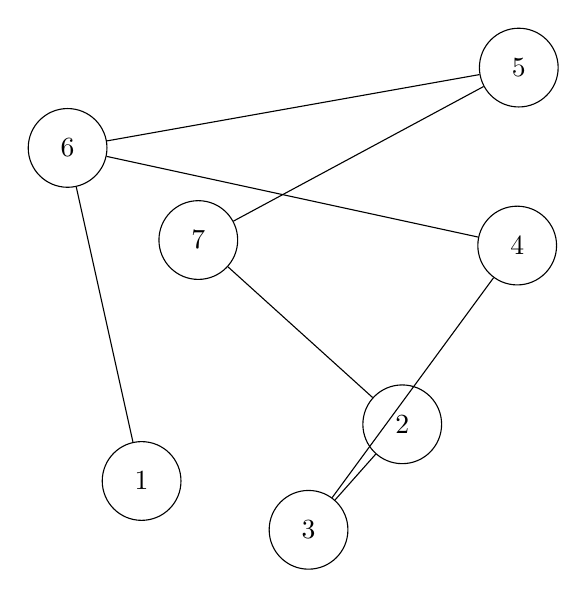
\begin{tikzpicture}[node distance=2cm, every node/.style={circle, draw, minimum size=1cm}]
  \node (1) at (-3.87, -2.90) {1};
  \node (2) at (-0.56, -2.18) {2};
  \node (3) at (-1.75, -3.52) {3};
  \node (4) at (0.90, 0.09) {4};
  \node (5) at (0.92, 2.35) {5};
  \node (6) at (-4.81, 1.33) {6};
  \node (7) at (-3.15, 0.16) {7};
  \draw (3) -- (4);
  \draw (6) -- (5);
  \draw (6) -- (4);
  \draw (5) -- (7);
  \draw (2) -- (3);
  \draw (7) -- (2);
  \draw (1) -- (6);
\end{tikzpicture}
\end{center}

\choice
{5}
{1}
{7}
{\True 1}
\loigiai{}
\end{ex}

\begin{ex}
Đồ thị bên dưới có mấy cạnh cầu?
\begin{center}
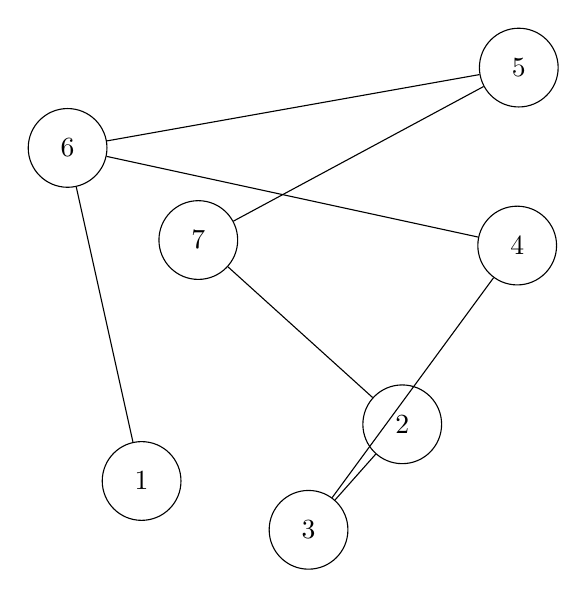
\begin{tikzpicture}[node distance=2cm, every node/.style={circle, draw, minimum size=1cm}]
  \node (1) at (-3.87, -2.90) {1};
  \node (2) at (-0.56, -2.18) {2};
  \node (3) at (-1.75, -3.52) {3};
  \node (4) at (0.90, 0.09) {4};
  \node (5) at (0.92, 2.35) {5};
  \node (6) at (-4.81, 1.33) {6};
  \node (7) at (-3.15, 0.16) {7};
  \draw (3) -- (4);
  \draw (6) -- (5);
  \draw (6) -- (4);
  \draw (5) -- (7);
  \draw (2) -- (3);
  \draw (7) -- (2);
  \draw (1) -- (6);
\end{tikzpicture}
\end{center}

\choice
{6}
{\True 1}
{2}
{4}
\loigiai{}
\end{ex}
\Closesolutionfile{ans}
\end{document}